\documentclass[letterpaper,10pt]{article}

\usepackage{titling}
\usepackage{listings}
\usepackage{url}
\usepackage{setspace}
\usepackage{subfig}
\usepackage{sectsty}
\usepackage{pdfpages}
\usepackage{colortbl}
\usepackage{multirow}
\usepackage{relsize}
\usepackage{amsmath}
\usepackage{fancyvrb}
\usepackage{amsmath,amssymb,amsthm,graphicx,xspace}
\usepackage[titlenotnumbered,noend,noline]{algorithm2e}
\usepackage[compact]{titlesec}
\usepackage[default]{droidserif}
\usepackage[T1]{fontenc}
\usepackage{tikz}
\usetikzlibrary{arrows,automata,shapes,trees,matrix,chains,scopes,positioning,calc}
\tikzstyle{block} = [rectangle, draw, fill=blue!20, 
    text width=2.5em, text centered, rounded corners, minimum height=2em]
\tikzstyle{bw} = [rectangle, draw, fill=blue!20, 
    text width=4em, text centered, rounded corners, minimum height=2em]

\definecolor{namerow}{cmyk}{.40,.40,.40,.40}
\definecolor{namecol}{cmyk}{.40,.40,.40,.40}

\let\LaTeXtitle\title
\renewcommand{\title}[1]{\LaTeXtitle{\textsf{#1}}}


\newcommand{\handout}[5]{
  \noindent
  \begin{center}
  \framebox{
    \vbox{
      \hbox to 5.78in { {\bf ECE155: Engineering Design with Embedded Systems } \hfill #2 }
      \vspace{4mm}
      \hbox to 5.78in { {\Large \hfill #4  \hfill} }
      \vspace{2mm}
      \hbox to 5.78in { {\em #3 \hfill} }
    }
  }
  \end{center}
  \vspace*{4mm}
}

\newcommand{\lecture}[3]{\handout{#1}{#2}{#3}{Lecture #1}}
\newcommand{\tuple}[1]{\ensuremath{\left\langle #1 \right\rangle}\xspace}

\addtolength{\oddsidemargin}{-1.000in}
\addtolength{\evensidemargin}{-0.500in}
\addtolength{\textwidth}{2.0in}
\addtolength{\topmargin}{-1.000in}
\addtolength{\textheight}{1.75in}
\addtolength{\parskip}{\baselineskip}
\setlength{\parindent}{0in}
\renewcommand{\baselinestretch}{1.5}
\newcommand{\term}{Spring 2014}

\singlespace

\begin{document}

\lecture{ 6 --- Events, Polling vs. Interrupts}{\term}{Jeff Zarnett \& Patrick Lam}

\section*{Event-Driven Programming}
We're going to talk about events in today's lecture, because we use
the \emph{event-driven paradigm} to receive sensor data in the labs.  Other programming paradigms for
embedded systems exist, e.g. the superloop structure.

Events are applicable to many application areas beyond embedded
systems, notably graphical user interfaces (e.g. mouse clicks,
keystrokes are typical events).

An \emph{event} is a notification of a change to the state of your system, such 
as a button click.

\begin{center}

\includegraphics{images/go-button}
\end{center}

Typically, you don't create events yourself; the system creates them
(perhaps in response to notifications from hardware devices---sensors,
timers, or the processor itself) and calls your \emph{event listener}, telling
you that an event occurred. You just wait for events to occur and react
to them. Event-driven software is reactive, not proactive:
traditionally, events come to you. This represents an 
inversion of control. (You may, however, schedule an event to be delivered
at some point in the future, which includes ``right now''.)



{\sf Why would you use an event-driven programming model?} \\[4em]
% can help you better structure your code
% more efficient when you have diverse event handlers rather than
%   looping through each possible event and checking to see if it happened

{\sf What are some real-life analogies to event-driven programming?}
~\\[4em]

%Analogy: you pay your bills only once the mail carrier brings them to 
%your door.

Here's how to do event-driven programming for the click event, then.
\begin{itemize}
\item To receive click events: 
\begin{itemize} \item the application registers an event 
listener with the object representing the button.\\
{\tt \qquad go.setOnClickListener(\ldots);}
\end{itemize}
\item When the user clicks the button: 
\begin{itemize}
\item the system executes the click event listener.
\end{itemize}
\end{itemize}

\paragraph{Implementing Event Listeners.}
We've seen that the application has to call {\tt setOnClickListener()} 
on the button. What does it pass to that method? A {\tt View.OnClickListener} object.

You could declare one:

{\small
\begin{minipage}{.5\textwidth}
\begin{verbatim}
class MyClickListener 
      extends View.OnClickListener {
  public void onClick(View v) {
    Log.d("A2", "clicked!");
  }
}
\end{verbatim}
\end{minipage}
\begin{minipage}{.5\textwidth}
\begin{verbatim}
// (somewhere else:)
go.setOnClickListener(new MyClickListener()); 
\end{verbatim}
\end{minipage}
}

But, there's a better way:

{\small
\begin{verbatim}
go.setOnClickListener(new View.OnClickListener() {
  public void onClick(View v) {
    Log.d("A2", "clicked!");
  }
  }); 
\end{verbatim}
}

This is called an \emph{inner class}.

\paragraph{Advantages of Inner Classes.}
\begin{itemize}
\item They don't litter your code with one-time-use classes.
\item They can access fields and (final) local variables.
\end{itemize}

{\small
\begin{verbatim}
class MainActivity {
  int i;

  @Override
  protected void onCreate(Bundle savedInstanceState) {
    Button go = (Button) findViewById(R.id.go);
    final int j = 2;
    go.setOnClickListener(new View.OnClickListener() {
      public void onClick(View v) {
        Log.d("A2", "i is "+i+" and j is "+j);
      }
      }); 
  }
}
\end{verbatim}
}

\paragraph{An Alternative to Inner Classes.}
You have another option. From the Android documentation~\cite{android:button}, you could use the following
in your Activity XML:
\begin{verbatim}
  <Button
     android:layout_height="wrap_content"
     android:layout_width="wrap_content"
     android:text="@string/self_destruct"
     android:onClick="selfDestruct" />
\end{verbatim}

Then, in your activity, you must include the method:
\begin{verbatim}
  public void selfDestruct(View view) {
     // Kaboom
  }
\end{verbatim}

\paragraph{Callback methods.} Applications sometimes need a particular
method to be called in the future. \emph{Callback methods} are a way of
implementing this design. For instance, event handlers should be called 
when the appropriate event occurs. 
One use of callback methods is to structure applications with 
time-consuming tasks:
\begin{itemize}
\item The application registers a callback to run upon completion (or
  near-completion) of the time-consuming task.
\item The application spawns the time-consuming task (perhaps in a
  different thread), and doesn't wait for it to finish.
\item The application continues normally, forgetting about the
  time-consuming task for now.
\item Once the time-consuming task finishes (or is about to finish),
  the callback executes, notifying the main application about the
  completion.
\end{itemize}
Callback methods therefore permit asynchronous (non-blocking) execution.

{\sf Can you name a real-life analogy to the workflow described above?}
\\[1em]

\paragraph{Synchronous vs. Asynchronous Execution.} The programs we've
seen so far are \emph{synchronous} (or sequential): each instruction
executes in sequence, and an instruction can only execute after its
predecessor completes.
In particular, when a program calls a function, it waits for the function
to return before continuing with its own execution, no matter how long
the function takes to complete.

Because the application is only doing one thing at a time, it is much
easier to understand than asynchronous programs.

It is also possible to write \emph{asynchronous} (or concurrent)
programs. In these programs, a main program may spawn a function, or
task, and continue executing before the function returns.

Writing asynchronous programs permits higher performance on modern
multi-core architectures; for some application domains, concurrency is
also a better way to structure the code.

\section*{Miscellaneous Comments about Events}
Here are a couple notes about events that you might want to know.

\paragraph{Priorities.} Some problems are more important to deal
with right away than others, e.g.:
\begin{itemize}
\item your mom calls; 
\item supper is burning; and
\item the laundry is done.
\end{itemize}
Which would you do first?

What about events with similar priorities? How would you choose?
Do you always need to choose?

Last time, I mentioned that we could put events into dispatcher queues.
Using the \emph{priority queue} data structure, the dispatcher
can efficiently pick out the highest-priority event and handle it first.

\paragraph{Events and finite-state machines.}
One way of implementing functionality in  event-driven software is via finite-state
machines (FSMs), containing an infinite loop between states. You'll
see FSMs in ECE124 this term. FSMs consume events and update system
state. You may choose to implement your signal processing code using an FSM.


% The objective of this lecture is to explain events in more detail.
% We'll talk about what events are and how they arise.
% This is the important notion of polling versus interrupts.

% Also make a link with Friday's lecture about CCR and handling events
% using dispatchers/arbiters.

% In the next lecture, we'll talk about how to handle events, using the
% C# notion of delegates.

\section*{Polling versus Interrupts}
For most of this course, you're just going to assume that events
come at you from nowhere. We'll briefly look at sources
of events to get a better understanding of event-driven
programming.

One source of events is through polling the sensors every so often; 
sensor readings then generate events.  Or, important events may
interrupt the processor to let you know about their existence.
It's also possible to use both polling and interrupts at the same time.

\subsection*{Polling} Polling means that the processor requests readings from
the device at its convenience. (e.g. what is the current light level?)
A polled device does not impose any schedule on the processor, so we
can call this \emph{passive synchronization}.


\noindent
When should a processor check device readings?

\begin{itemize}
\item whenever convenient (occasional polling);
\item at fixed time intervals (periodic polling);
\item constantly (tight polling).
\end{itemize}

Any of these strategies may be appropriate (with different constants),
depending on the importance of the event and the frequencies at which
events occur.

\vspace*{-1em}
\paragraph{Digression: Input/Output.} Recall this picture from lecture 1:

\begin{center}
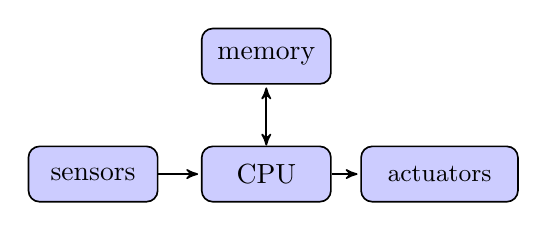
\begin{tikzpicture}[->,>=stealth',shorten >=1pt,auto,node distance=2.2cm,
                    semithick,initial text=]
  \node[bw]   (cpu)               {CPU};
  \node[bw, left of=cpu] (sensors) {sensors};
  \node[bw, right of=cpu, text width=5em] (actuators) {\small actuators};
  \node[bw, above of=cpu,yshift=-2em] (memory) {memory};

  \path (cpu) edge[<->] node {} (memory)
        (sensors) edge node {} (cpu)
        (cpu) edge node {} (actuators);
\end{tikzpicture}
\end{center}

How does the CPU actually talk to the sensors and actuators?  Two
methods: 1) memory-mapped I/O and 2) port-mapped I/O, or special
instructions.  In memory-mapped I/O, the CPU executes what it thinks
are reads and writes to memory. In particular, it sends out the
appropriate requests on the system bus. Devices listen on the bus and
manufacture the appropriate responses. For special instructions, as seen
on Intel ia32 processors, the CPU instead executes special {\tt in} and
{\tt out} instructions, which may transmit data on a special bus,
or set a specific signal on the bus.

\paragraph{Pseudocode for Tight Polling Loop.} 
Here is pseudocode for a memory-mapped I/O system.
%	// Read a status register to check for a new event
%	// A statusRegister value of 0x0000 indicates no event has occurred.  The value of the statusRegister
%	// variable will change to a non-zero value when an event has occurred.
\begin{verbatim}
        while( statusRegister == 0x0000 ) {
            // Do nothing until statusRegister changes value
        }
        //  Read data that has changed from a dataRegister and store in memory
        incomingData = dataRegister;
\end{verbatim}
We'd expect this loop to terminate based on some hardware specification
promising {\tt statusRegister} eventually becoming non-zero due to an
external event. Data exchange occurs once the device indicates that
it is ready to emit data (by setting {\tt statusRegister}); we can
call this \emph{polling synchronization}.

% mention memory-mapped registers

\subsection*{Interrupts}
\vspace*{-1em}
\hfill \emph{``In Soviet Russia, event polls you.''}

Another way that a processor can find out about an event is via an
\emph{interrupt}. Interrupts \emph{actively synchronize} a device and
a processor.  An interrupt tells the processor one bit of information:
that something worth knowing about (high-priority) is occurring. When
the processor gets an interrupt, it stops what it's currently doing,
saves its state, and starts executing a pre-defined \emph{interrupt
  handler}.  The interrupt handler will typically read the event
information (how?) and store it somewhere accessible.  After the handler
returns, the processor restores its state and resumes what it was
doing before.

% real-life analogy: phone calls

\section*{Inversion of Control}
As we talked about last time, Android programming is event-driven programming,
which changes the basic structure of a program from what you saw in ECE150.

Here's a representation of how a program works, as you saw it in ECE150:

\begin{center}
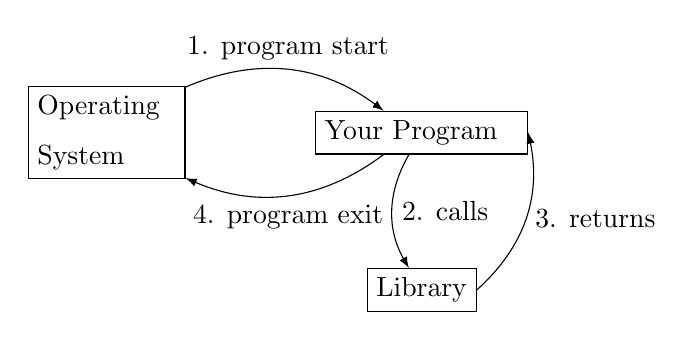
\begin{tikzpicture}
\path (0, 0) node[draw,text width=5em] (OS) { Operating System }
    +(4, 0) node[draw, text width=7em] (you) {Your Program};
\path (4, -2) node[draw] (lib) {Library};

\path[->,bend left,>=latex] (OS) edge node[above] {1. program start} (you);
\path[->,bend left,>=latex] (you) edge node[below] {4. program exit} (OS);
\path[->,bend right,>=latex] (you) edge node[right] {2. calls} (lib);
\path[->,bend right,>=latex] (lib.east) edge node[right] {3. returns} (you.east);
\end{tikzpicture}
\end{center}

The main idea is that when the user chooses to launch your program,
you have all the control until you exit. If you want some input, you'll ask
the library/operating system for the input (using a system call), and
it'll return it to you when it returns. 

Note that calling the library does not lead, by itself, to an inversion of control.

\paragraph{New Event-Driven Paradigm.} Here's an example of the new paradigm.

\begin{center}
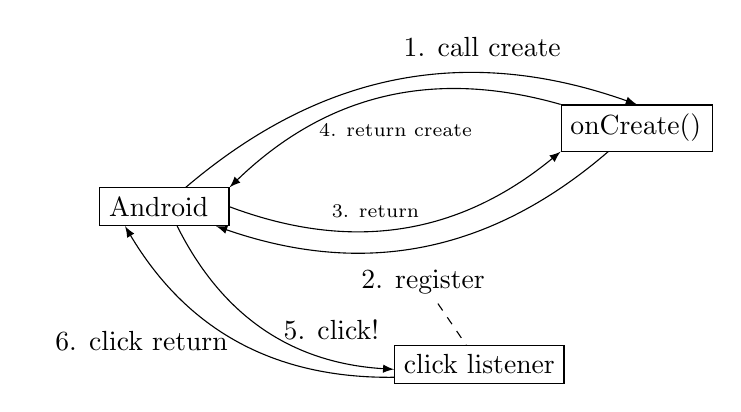
\begin{tikzpicture}
\path (0, 0) node[draw,text width=4em] (OS) { Android }
    +(6, 1) node[draw, text width=4.8em] (you) { onCreate() };
\path (4, -2) node[draw] (listener) {click listener};

\path[->,bend left,>=latex] (OS) edge node[above,yshift=0.5em, xshift=3em] {1. call create} (you.north);
\path[->,bend left,>=latex] (you) edge node[below,name=reg,yshift=-.5em] {2. register} (OS);
\path[dashed] (reg) edge (listener);
\path[<-,bend left,>=latex] (you.south west) edge node[above,xshift=-1em,name=reg] {\scriptsize 3. return} (OS.east);
\path[->,bend right,>=latex] (you.north west) edge node[above,at end,xshift=6em,yshift=1.5em] {\scriptsize 4. return create} (OS.north east);
\path[->,bend right,>=latex] (OS) edge node[right] {~5. click!} (listener);
\path[<-,bend right,>=latex] (OS.south)+(-0.5,0) edge node[left] {~~6. click return} 
                                 (listener)+(1,0);
\end{tikzpicture}
\end{center}
Now, Android takes all of the responsibility for calling your code when appropriate.
It'll start your Activity by calling the {\tt onCreate()} method. In that method,
you may choose to register event listeners, or programmatically add widgets. But you
only do setup work there. Don't do any real computation.

Next, when something happens, Android is going to call you and let you know about it.
It's doing something that looks like this:

\begin{verbatim}
while (!done) {
 r <- fetch Runnable from Queue
 dispatch r
}
\end{verbatim}

This is like a tight polling loop, but it goes to sleep between events (in the
fetch).




\bibliographystyle{alpha}
\bibliography{155}


\end{document}
